\section{Incremental Clustering}
\label{sect:incremental-clustering}

The incremental clustering phase translates changes of the input graph to changes of the cluster graph formed from the input graph in an earlier step of the pipeline. Recall that the cluster graph is passed as an input to this phase to ensure that the produced sequence of operations is applicable to the cluster graph that has already been locked in in an earlier run through the pipeline. Also note that the produced sequence of operations on the cluster graph potentially is empty.

\begin{figure}[H]
	\centering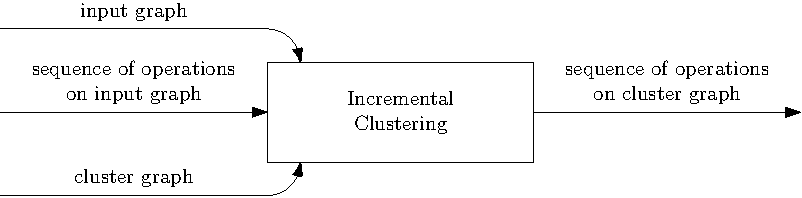
\includegraphics[width=0.8\textwidth]{Resources/DynamicPipeline-IncrementalClustering.pdf}
	\caption{Input and output of the incremental clustering phase.}
	\label{fig:dynamic-pipeline-incremental-transformation}
\end{figure}

We assume that in concrete implementations, the cluster graph preserves enough information about the input graph it was formed from to allow for proper incremental clustering. For example, the cluster graph might keep track of which vertices of the input graph its clusters contain, such that cluster weights can be adjusted or clusters can be split accordingly.

Our pipeline supports the following class of primitive operations on cluster graphs:
%
\begin{itemize}
	\item \textbf{Insert vertex:} As new clusters appear in the input graph, corresponding vertices can be added to the cluster graph along with edges to the existing vertices. The weights for the new vertices and edges can be chosen arbitrarily.
	\item \textbf{Remove vertex:} As clusters in the input graph cease to exist, the corresponding vertices in the cluster graph can be removed along with any incident edges.
	\item \textbf{Update vertex weight:} As a cluster in the input graph grows or shrinks, \ie{} vertices are added to or removed from it, existing vertices' weights can be set to an arbitrary new values.
	\item \textbf{Update edge weight:} As the similarity between two clusters in the input graphs grows stronger or weaker, existing edges' weights can be set to arbitrary new values.
\end{itemize}
%
Note that because the cluster graph is a complete graph, we are not allowed to add or remove individual edges and adding a new vertex to the cluster graph implicitly adds edges to all existing vertices. However, edges are allowed to have a weight of zero.

More complex changes of the input graph, such as two clusters merging or separating, can be expressed as a sequence of operations listed above. In fact, these operations are sufficient to convert between arbitrary cluster graphs $G_0$ and $G_i$, \ie{} no matter what cluster graph $G_0$ the non-incremental clustering phase originally produced, it can still be turned into any other cluster graph $G_i$ by gradually incorporating changes of the input graph.
